% Collapsing X^n/X^{n-1}: the pair (X,A) of two triangles becomes a
% wedge of two 2-spheres joined at the point A/A.
% Source: book/tex/homology/cellular.tex (§ Cellular chain complex).
\documentclass[border=2mm]{standalone}
\usepackage{tikz}
\usepackage{amssymb}
\usetikzlibrary{arrows.meta}
\begin{document}
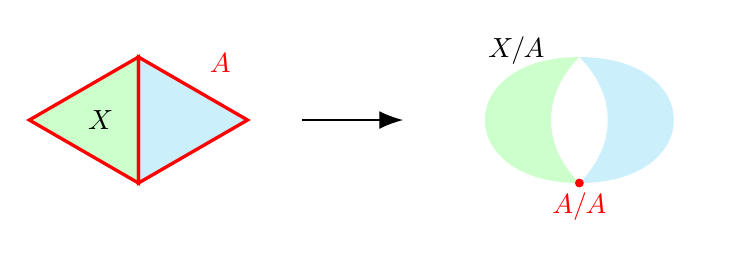
\begin{tikzpicture}[scale=0.8]
  % Left: pair (X, A), two triangles sharing the red edge A.
  \fill[cyan!20] (-4,1) -- (-4,-1) -- (-4+1.732,0) -- cycle;
  \fill[green!20] (-4,1) -- (-4,-1) -- (-4-1.732,0) -- cycle;
  \draw[red, line width=1.2pt] (-4,1) -- (-4,-1) -- (-4+1.732,0) -- cycle;
  \draw[red, line width=1.2pt] (-4,1) -- (-4,-1) -- (-4-1.732,0) -- cycle;
  \node at (-4.6,0) {$X$};
  \node[red] at (-2.7,0.9) {$A$};
  % Arrow.
  \draw[-{Latex[length=3mm]}] (-1.4,0) -- (0.2,0);
  % Right: wedge of two spheres (blobs) at A/A.
  \fill[cyan!20] (3,-1) .. controls (5,-1) and (5,1) .. (3,1) .. controls (3.6,0.4) and (3.6,-0.4) .. (3,-1);
  \fill[green!20] (3,-1) .. controls (1,-1) and (1,1) .. (3,1) .. controls (2.4,0.4) and (2.4,-0.4) .. (3,-1);
  \node at (2,1.1) {$X/A$};
  \fill[red] (3,-1) circle (2pt) node[below, red] {$A/A$};
\end{tikzpicture}
\end{document}
